\documentclass{article}
\usepackage{algorithmicx}
\usepackage{algpseudocode}
\usepackage{graphicx}
\usepackage{color}
\usepackage[utf8]{inputenc}

\begin{document}
{\noindent \Huge Problema a resolver:}
\newline \newline  El problema esta dado por la siguiente situaci\'on: 
tenemos en un $"$lista$"$ con una cantidad \textit{3$*$n} de n\'umeros(n un n\'umero fijo).\newline
Para \textit{i} desde \textit{0} a \textit{n-1}, vamos a decir que la posici\'on \textit{i} en la lista va a ser \textit{Izq} del edificio \textit{i-\'esimo}, \textit{i+1} va a ser \textit{Alt} del edificio \textit{i-\'esimo} e \textit{i+2} va a ser \textit{Der} del edificio i-\'esimo.\newline
A grandes rasgos vamos a tener una lista de \textit{n} edificios (interpretamos a un edificio como una tupla \textit{$<$Izq,Alt,Der$>$}) con una base en com\'un impl\'icita que es 0.\newline
Vamos a utilizar esta notación para referirnos a los edificios.\newline
Por ejemplo para un entrada de la forma: \newline
\textit{lista={1,2,3,4,2,7,2,4,6}} y 
\textit{n=3} tendr\'iamos: \newline 
\textit{lista$=$ $<$1,2,3$>$,$<$4,2,7$>$,$<$2,4,6$>$} proyectada en un gr\'afico quedar\'ia: \newline
\vspace{0.4cm}
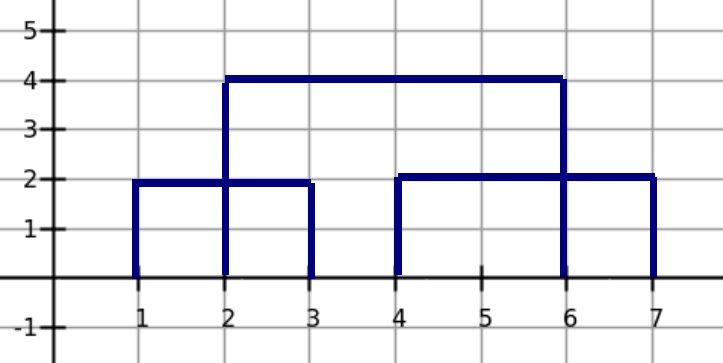
\includegraphics[width=\textwidth,height=\textheight,keepaspectratio
]{edificiosGraf1.png}
\begin {flushleft}
\end{flushleft}

Lo que queremos hacer es $"$eliminar todas las lineas interiores del gr\'afico$"$, quedarnos con su contorno (se obtiene el mismo resultado  "siguiendo con el dedo el gr\'afico") para luego poder dar la solución final que explicaremos más adelante. \newpage
Veamos un ejemplo de eliminación de lineas interiores y el "procedimiento" de seguir con el dedo el gráfico \newline
Para una \textit{lista$=$ $<$0,3,8$>$,$<$1,6,5$>$,$<$2,4,6$>$,$<$4,2,7$>$,$<$9,6,10$>$} con \textit{n=5},\newline su gr\'afico es: \newline
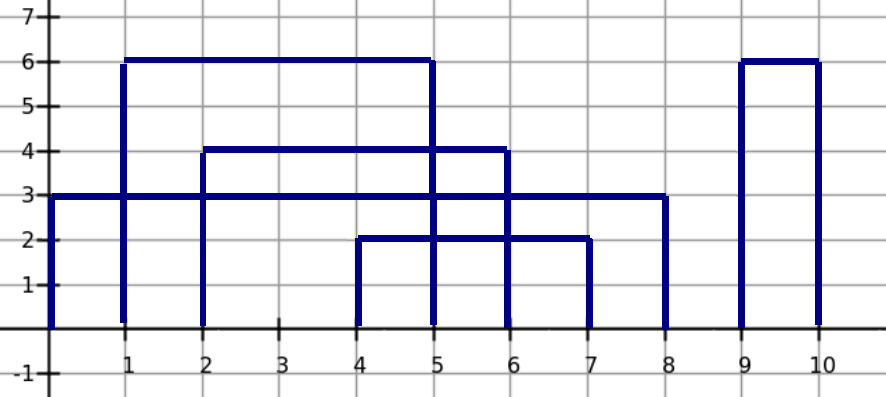
\includegraphics[width=\textwidth,height=\textheight,keepaspectratio
]{edificiosGraf2.png}
\begin {flushleft}
\end{flushleft}

el gr\'afico de eliminar las lineas interiores es:\newline
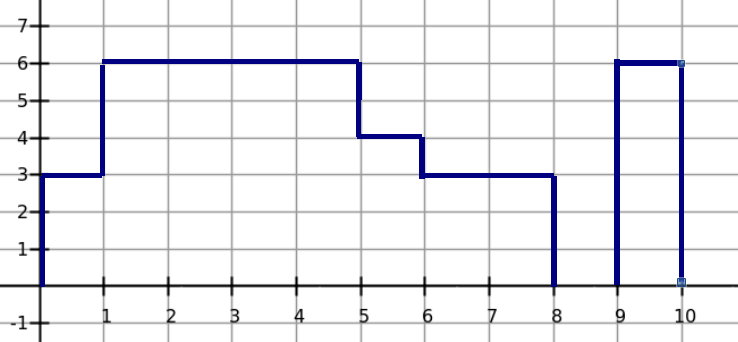
\includegraphics[width=\textwidth,height=\textheight,keepaspectratio
]{edificiosGraf2b.png}
\begin {flushleft}
\end{flushleft}
\newpage
Mientras que el gr\'afico de "seguir con el dedo" es: \newline
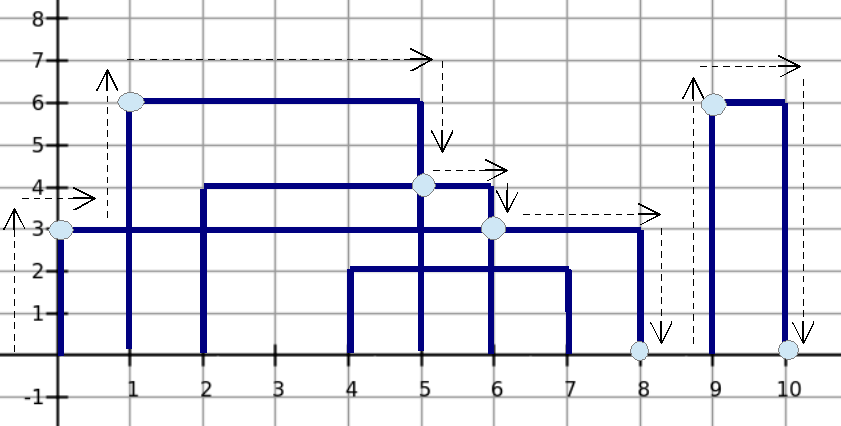
\includegraphics[width=\textwidth,height=\textheight,keepaspectratio
]{edificiosGraf2c.png}
\begin {flushleft}
La salida para este ejemplo  \textit{{0,3,1,6,5,4,6,3,8,0,9,6,0}}
\end{flushleft}

Lo que hago cuando "sigo con el dedo" es: \newline
Empezar con el primer edificio y seguimos el trazo, si me interseco con otro edificio seguir el trazo del edificio con el que me intersequ\'e desde ese punto. \newline
Si no me interseco con nadie pero hay m\'as edificios adelante "siguir con el dedo" los otros. Si no hay más edificios termin\'e.\newline
Luego de ese contorno voy a obtener la soluci\'on final que son los puntos donde hay cambios de altura($\uparrow$ $\longrightarrow$ y $\downarrow$ $\longrightarrow$). \newline

\newpage

{\noindent \Huge Resoluci\'on:}
\newline \newline
Un panorama de la resolución es:\newline
ordenar los edificios de menor a mayor por su Izq (en caso que tengan la misma izquierda es menor el que tiene mayor altura). \newline
Retornar el primer punto del primer edifico de la lista de edificios ordenada. \newline
Vamos recorriendo los edificios(mirando el edificio por el que voy ,anterior, y uno mas adelante,siguiente).\newline
Si anterior interseca a siguiente, encolo anterior y retorno el cambio de altura si siguiente es mayor en altura que anterior.\newline
Si es igual en altura o mayor, ahora anterior es siguiente. Si es menor en altura no hago nada. \color{red}{no vale la pena ponerlo} \newline \color{black}{}
Encolo anterior en la cola y sigo iterando.
Si anterior no interseca a siguiente(quiere decir que están "separados",pero puede que antes de anterior haya un edificio que termine después que anterior, empiece antes que anterior y sea menor en altura )
voy a buscar este edificio en la cola (ordenada por altura) desencolando y mirando el tope:\newline
si lo encuentro, ese edificio ahora es anterior, retorno la intersección.\newline
si la cola es vacía(quiere decir que no había ningún edificio que terminara después que anterior) retorno anterior.Der,0,siguiente.Izq,siguiente.Alt y ahora anterior es siguiente.
\newline
Terminé de recorrer los edificios,pero puede que hayan quedado cosas dentro del heap, y son puntos que debería tener la solución
Mientras el heap tenga edificios, voy a comparar el tope con anterior:\newline
si tope termina antes que el anterior desencolo, en caso contrario retorno la intersección. 
Ahora anterior es el toper de la cola y desencolo.\newline
Ya no hay más nada en el heap, \color{red}{mirar} \color{black}
\newline
Hay cosas que en esta descripción no tuve en cuenta, porque son muy especificas, para explicarlo profundamente lo hago con este pseudocódigo: 
\newline
 
Sea lista: lista($<$Izq,Alt,Der$>$) y n la cantidad de tuplas en la lista.


\vspace{0.4cm}
\begin{algorithmic}[1]
\Procedure{ResolverEdificios}{$lista$,$n$}
	\State $\textit{ordenar los edificios por Izq}$
	\State $comparo\gets lista[0]$
	\State $cola\gets vacio$
	\State $\textit{imprimo el primer punto(comparo.Izq y comparo.Alt)}$
	\For{$(i\gets 1, n-2)$} \textit{$//$voy recorriendo los edificios hasta el anteúltimo, \color{red}{si hay 0 edificios que hago?} \color{black}}
		\State $siguiente\gets lista[i]$
		\If{$(\textit{se intersecan comparo y siguiente\color{red}{*0}})$}
			\If{$(\textit{siguiente $>$ comparo en altura \color{red}{*1}})$}
				\State $\textit{imprimir cambio de altura}$
				\If{$(\textit{la cola está vacia})$}
					\State $\textit{cola.encolar(comparo)}$
				\Else
					\If{$(\textit{comparo no está en el tope de la cola}$)}
					\State$\textit{cola.encolar(comparo)}$						
					\EndIf			
				\EndIf
					\State $comparo\gets siguiente$
			\EndIf
			\If{$(\textit{siguiente $==$ comparo en altura \color{red}{*2}})$}
				\If{$(\textit{la cola está vacia})$}
					\State $\textit{cola.encolar(comparo)}$
				\Else
					\If{$(\textit{comparo no está en el tope de al cola}$)}
					\State$\textit{cola.encolar(comparo)}$
					\EndIf			
				\EndIf
			\EndIf
			\If{$(\textit{siguiente $<$ comparo en altura \color{red}{*3}})$}
				\State $cola.encolar(siguiente)$
			\EndIf
			
		\EndIf \textit{(no se intersecan comparo y siguiente\color{red}{*4})}
		\If{$(\textit{la cola no está vacia})$}
			\While{$(\textit{cola no vacia})$}
				\If{$(\textit{primero.cola termina antes que comparo \color{red}{*5}})$}		
				\State $\textit{desencolar.cola}$
				\Else \textit{(primero.cola termina despues que comparo \color{red}{*6})}
				\State $\textit{imprimir interseccion entre comparo y primero.cola}$
				\State $comparo\gets primero.cola$
				\State $\textit{desencolar.cola}$
				\EndIf
			\EndWhile
		\Else{\textit{ //no pasé a nadie que cortaría a comparo, como no se intersecan imprimo ambos puntos}}
		\State $\textit{imprimir comparo.Der y 0 }$
		\State $\textit{imprimir siguiente.Izq y siguiente.Alt}$
		\State $comparo\gets siguiente$
		\EndIf
	\EndFor{\textit{(no hay siguiente,puede que hayan quedado cosas en el cola \color{red}{*7}})}
	\textit{//uso a comparo que es el último edificio visto con el que haya en el tope de la cola}
	\For{$(\textit{la cola no es vacia}, \textit{desencolar})$}
	\If{$(\textit{comparo termina antes que primero.cola \color{red}{*8})}$}
		\State $\textit{imprimir intersección comparo y primero.cola}$
		\State $comparo\gets cola.primero$
	\EndIf
	\EndFor{(\textit{al último punto no lo imprimo nunca\color{red}{*9})}}\newline
	\textit{$//$lo imprimo acá}
	\State $\textit{imprimir comparo.Der y 0}$
\EndProcedure
\end{algorithmic}

\newpage

{\noindent \Huge Complejidad:}
\newline \newline
Vamos a ver que la cantidad de veces que encolo es una funcion de n, y así poder ver que la cantidad de veces que desencolo es tambien una funcion de n porque no puedo desencolar más cosas de las que encolo.
Vemos en el algoritmo que en  *1 y *2,encola si está vacia y si el elemento está en el tope, no lo encolo.(\color{red}{falta demostrar que si quiero encolar un elemento 2 veces el que quiero encolar de nuevo está en el tope, la idea la había sacado angel})\color{black} Luego en *3 encolo. Despues a lo largo de todo el algoritmo no hago \textit{nunca} un encolar
Como todos estos casos son disjuntos (o son $<$,$>$ o $=$ las alturas de comparo y siguiente) entonces hago 1 encolar en cada edificio en peor caso, con lo cual hago n encolar. 
\newline

Veamos ahora la complejidad del while dentro del for(de recorrer los edificios), en peor caso por cada edificio desencolo todos los edificios eso da una complejidad n*(n*log(n)), pero si analizamos más finamente, nunca podría para cada paso desencolar todos los edificios.\newline
Si voy por el edificio \textit{i} (\textit{i} entre \textit{0} y \textit{n-1}), tengo en el heap en peor caso \textit{i} edificios(por lo explicado arriba de la cantidad de encolar), entro en el while(suponiendo que los edificios \textit{i} e \textit{i+1} no se tocan) y desencolo \textit{i} edificios(en peor caso desencolo todos los que encolé), sigo avanzando y llego a un edificio \textit{j} (\textit{j} entre \textit{0} y \textit{n-1} y es mayor que \textit{i}) ahora en el heap en peor caso tengo \textit{j-i} edificios(pues los edificios anteriores a \textit{i} ya no están en la cola y encolé todos desde \textit{i} hasta \textit{j}), entro en el while(suponiendo que los edificios j y j+1 no se tocan) y desencolo en peor caso \textit{j-i} edificios.
llego al último edificio \textit{n-1} y en peor caso tengo \textit{n-1- j} edificios en el heap(generalizando lo anterior), entro al while y desencolo \textit{n-1-j} veces.
Si sumo la cantidad de veces que hice desencolar en el recorrido lineal es n (suma de los intervalos).
Entonces hago n veces desencolar

Relacionando la parte de encolar y desencolar en el primer for
por cada edificio hago un encolar y una cantidad x de desencolar + c(\textit{constante}) operaciones que tienen costo 1 (asignaciones y guardas)
Por lo visto anteriormente la suma de esos x es n, entonces el costo es  n*(costo de encolar)+ n*(costo de desencolar) +c(constante)
\newline\
Solo nos falta analizar el segundo for(cuando salgo del primero), en peor caso tengo todos los edificiosque es  n, y desencolo hasta que se vacia,entonces hace n*(costo de desencolar) + c1(constante de guardas y asignaciones))
En la implementación usamos una priority-queue como cola, el costo de encolar(push) es log(n),desencolar(pop) es log(n) y tope(top) es 1.
\newline
Al princio del algoritmo ordeno los edificios por Izq, el costo de ordenarlos es n*log(n) (porque uso sort de la stl \color{red}{según este link} \color{black}).\newline

Finalmente la complejidad es \newline
O(n*log(n) de ordenarlos \newline
+ c[\textit{constante}]+n[\textit{encolar}]+n*(log(n))[\textit{desencolar}] del primer for \newline
+ c1[\textit{constante}] + n*log(n)[\textit{desencolar}] del segundo for)  $\in$ O(n(log(n))) \newline
\newpage



{\noindent \Huge Correctitud:}
\newline \newline
El algoritmo pone como primer "punto" la esquina izquierda(esquina izquierda gráfico) del primer edificio.\newline
En la solución("real", no de mi algoritmo) el primer "punto" es la esquina del edificio que tiene menor izquierda y mayor altura que todos.\newline
\color{red}{demo} \color{black}\newline
¿El primer punto que pone mi algoritmo cumple con dichas propiedades?
Veamos, ordeno los edificios por Izq de menor a mayor y en caso de tener el mismo Izq es menor el que tiene mayor altura(linea 2),
entonces el primer edificio va a ser el de menor izq y el de mayor altura.\newline
Con lo cual si,el primer punto cumple con las propiedades.
\newline

Voy iterando los edificios mirando el edificio por el que voy(comparo) y el siguiente. Comparo no necesariamente es uno menos que siguiente.

Si comparo y siguiente se intersecan(graficos intersecciones):\newline
	si comparo es menor a siguiente (grafico A)\newline
		tengo que poner el punto de intersección en la solución\newline
		Supongamos que ese punto (intersección) no es solución:\newline
			caso existe un edificio que empieza entre la Izq de comparo y la Izq de siguiente, termina después que Izq de siguiente y tiene altura mayo a comparo (ejemplo gráfico B):\newline
			si existiera este edificio tendría que ser haberlo puesto como siguiente cuando recorría los edificios , ABS!!!\newline
			Entonces el punto es solución.\newline
			caso exite un edificio que empieza antes que Izq de comparo, tiene Alt mayor que comparo y termina después que Izq de siguiente (ejemplo grafico C):\newline
			Si existiera tendría que haberlo puesto como anterior cuando recorria los edificios, ABS!!!\newline
			Entonces el punto es soución.\newline

Si no se intersecan comparo y siguiente(grafico no se intersecan):\newline
	voy a tener en el heap los edificios que terminan después que Izq de comparo porque los fui enconlando (grafico D)
	si el heap está vacío quiere decir que no hay nadie que corte a anterior(heapVacio grafico),entonces el edificio anterior sigue hasta su base y tengo que seguir con los demás edificios(en caso de tener más) desde siguiente, entonces voy a poner en la solución, el final de comparo y el principio de siguiente.\newline
	Si el heap no está vacío quiere decir que puede que tenga un edificio que corte a anterior (grafico corte anterior)
		voy a sacar del heap hasta que encuentro uno que interseque a anterior, por como es el heap (es un max heap en la altura) este que me interseca es el que tiene mayor altura, entonces este punto de intersección es solución.\newline
		Supongamos que este punto de intersección no es solución.\newline
		caso (grafico E) exite un edificio que empieza antes que Izq de comparo , termina despues que Der de comparo estricto y tiene altura entre altura de comparo y altura del tope del heap, entonces este si exitiera, lo tendría que haber encolado cuando recorría los edificios y tendría que ser el edificio que me daría el heap ABS!!!\newline
Entonces es solución.\newline

Siempre recorro los edificios mirando comparo y siguiente, en algún momento me voy a quedar sin edificios, comparo va a quedar en algún edificio y el heap va a tener algún estado (vacío o con edificios dentro)
Ahora voy a trabajar con comparo y el heap (ahora en el heap están mis "siguientes nuevos")
Si hay edificios en el heap: \newline
Pueden pasar 2 cosas que el siguiente del heap interseque en derecha a comparo (grafico interseque en derecha) o no: \newline
Primer caso, el punto de intersección es solución. \newline 
Supongamos que no lo es, entonces exites un edifcio que empieza antes que Izq del tope del heap, tiene mayor altura que el tope del heap y termina después que comparo, ABS!!!, porque si existiera lo tendría que haber encolado cuando recorría los edifcios y tendría que ser ese edificio el que me daría el heap.
Entonces es solución, ahora el tope del heap es comparo y desencolo.
Segundo caso, no me importa porque no hay posible solución, sigo desencolando.

En algún momento voy a terminar de vaciar este heap pero como nunca pongo puntos "por derecha" (gráfico de puntos por derecha), el último ediicio (el que termina último) va a estar en comparo.
¿Por qué? Pueden pasar 2 cosas:
 primero que comparo sea el último y tenga todas cosas en el heap que no corten por derecha a comparo, entonces las voy a desencolar todas y terminar, pero el punto "por derecha" de comparo nunca se retornó
 segundo comparo no sea el último, entonces el último va a ser uno del heap, cuando los voy desencolando y no tenga más cosas en el heap, comparo va a ser el que termina último y tiene mayor altura(porque pongo a siguiente en comparo cuando tengo que bajar REFINAR ESTO)
Entonces en ambos casos el edifcio comparo es el que termina último.
Luego de desencolar todas los del heap en el segundo for, mi algoritmo retorna el "punto por derecha " de comparo y un 0.




 
		
	\color{red}{NO ME GUSTA NADA ESTA DEMO! igual no es la final}\color{black}

\end{document}